%%=============================================================================
%% Methodologie
%%=============================================================================

\chapter{\IfLanguageName{dutch}{Methodologie}{Methodology}}
\label{ch:methodologie}

In dit hoofdstuk wordt uitgelegd hoe het toegepaste onderzoek wordt uitgevoerd. Met name, controleren in welke mate een specifieke organisatie (=Insites Consulting) reeds GDPR-compliant is. Er wordt bekeken welke stappen, software-gewijs, nog ondernomen moeten worden. 



\section{Overlopen bulletpoints}
De eerste stap om GDPR compliant te worden is niet de meest igewikkelde, maar des te belangrijk. Stel aan de hand van de uitleg in 'stand van zaken' een lijst op met alle acties die een organisatie kan ondernemen om te voldoen aan de regelgeving. Leg die lijst naast de werking van je organisatie, en beslis wat er kan verbeterd worden, hoe de zaken die nog niet compliant zijn, in volgorde van belang, kunnen opgelost worden.  

\subsection{Data Protection}

%% TODO: Hoe ben je te werk gegaan? Verdeel je onderzoek in grote fasen, en
%% licht in elke fase toe welke stappen je gevolgd hebt. Verantwoord waarom je
%% op deze manier te werk gegaan bent. Je moet kunnen aantonen dat je de best
%% mogelijke manier toegepast hebt om een antwoord te vinden op de
%% onderzoeksvraag.

\subsection{}
Uit dit onderzoek bij InSites Consulting blijkt dus dat ze als organisatie de vraag van een gebruiker om al zijn gegevens niet tot in de puntjes kunnen uitvoeren. Zijn hier mogelijkheden om dat te verbeteren? Dit zien we in punt 2. 

\section{Cognitive Services}
In dit onderdeel van het onderzoek wordt bekeken of het mogelijk is om persoonlijke data te gaan filteren uit open velden waar gebruikers mogelijks persoonlijke informatie achtergelaten hebben. 

\subsection{Azure Api }

\begin{figure}[h]
	\centering
	\begin{subfigure}{0.45\textwidth}
		\centering
		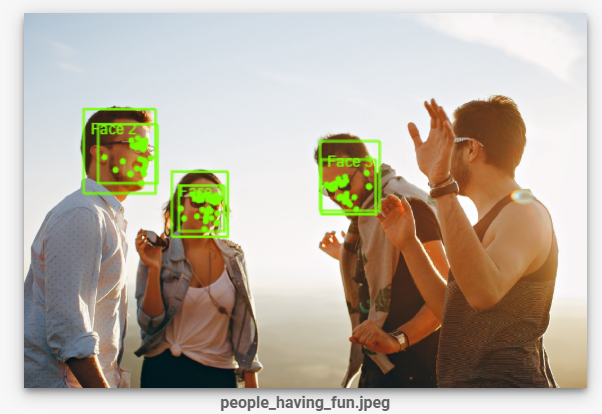
\includegraphics[width=.7\linewidth]{Face_recogn_google1.png}
		\caption{Google cloud}
		\label{fig:sub1}
	\end{subfigure}%
	\begin{subfigure}{0.45\textwidth}
		\centering
		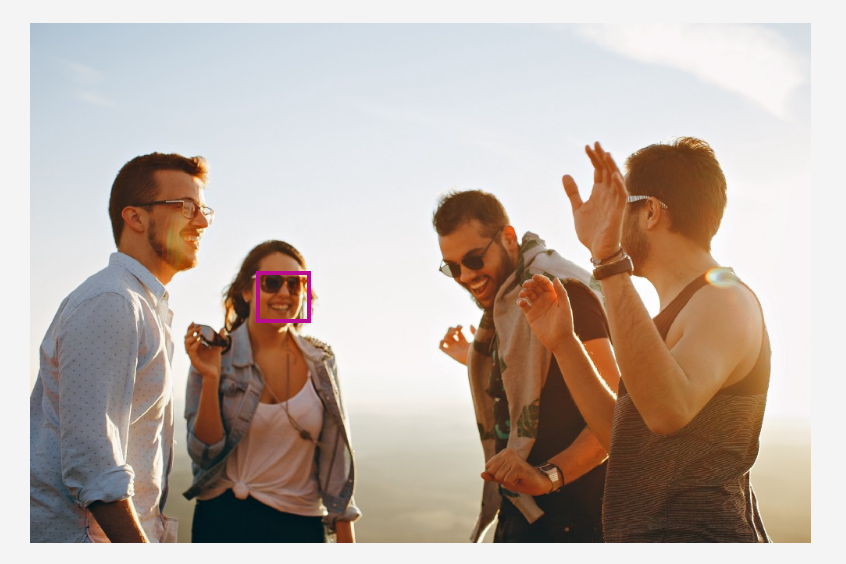
\includegraphics[width=.7\linewidth]{Face_recogn_micros_3.PNG}
		\caption{MS Cognitive Services.}
		\label{fig:sub2}
	\end{subfigure}
	\caption{Eenzelfde foto geïnterpreteerd door beide demo's. Google cloud herkent alle 3 de zichtbare gezichten, terwijl bij MS slechts één van de drie gezichten gevonden wordt.}
	\label{fig:test}
\end{figure}

\begin{figure}[h]
	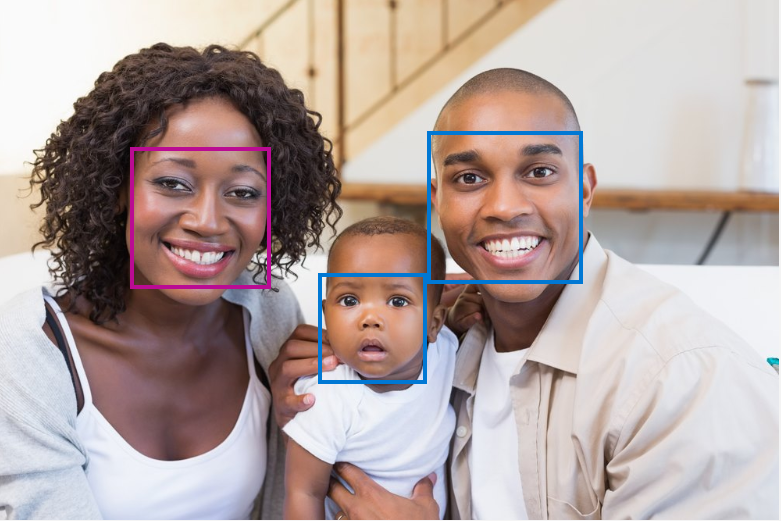
\includegraphics[width=\linewidth]{Face_recogn_micros_2.png}
	\caption{Cognitive services - Face recognition. Links de foto, rechts een JSON-file met herkende elementen.}
	\label{fig:cognitive2}
\end{figure}

[21-25]

